\section{Closure}
\label{sec:closure}

The aim of this section is to present results relating to the estimators in
section \ref{sec:estimators} and start the discussion for plan with regards
to future closure tests.

\subsection{Introduction}

We have seen that some examples of the strange behaviour that can arise when one
performs a naive hyperoptimization without a test set. Resulting
architecture/methodologies are capable of producing strange PDFs, one such
example is given in figure \ref{fig:v3pdf}

\begin{figure}[!h]
    \centering
    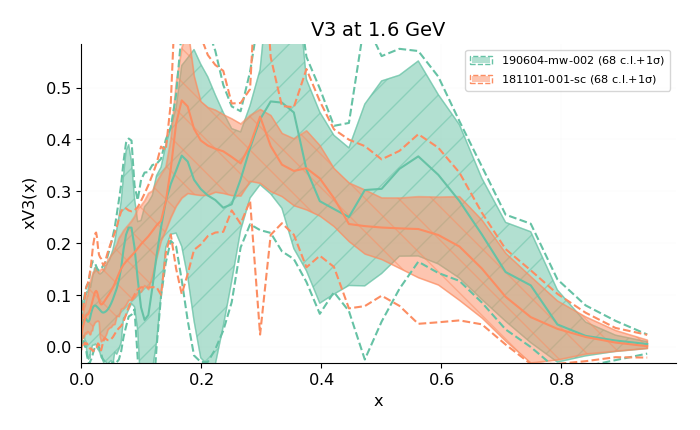
\includegraphics[width=0.8\textwidth]{plot_pdfs_V3.png}
    \caption{
        Figure showing wiggly behaviour of v3 PDF when using the new fitting code.
        }
    \label{fig:v3pdf}
\end{figure}

This leaves us with a few questions: Can we discriminate against this
architecture/minimiser choice in a closure test using the closure estimators?
Hopefully the answer is yes.

\subsection{results}

\subsubsection*{Closure on pseudodata from large architecture PDF}

As a sanity check we can run a closure test with the higher parameterisation
which gave wiggly PDFs in a fit to pseudo data which is generated from the
wiggly PDF. This is to see if the features we see in the space of the PDF are
somehow picked up by the data in such a way that we can refit the same underlying
function.

This is a brute force way of trying to understand whether the features in the PDF
are just flat directions in the loss or are some kind of feature of the data. To
test this I am taking as input a wiggly PDF, and then just generating the MC
replica (level 2) noise on top of this, and so there is no level 1 fluctuation.
The test is to see if the functional form of the replicas matches the input PDF.

The full report comparing the closure fit to underlying can be found here:
\href{https://vp.nnpdf.science/tHdjyBVTQEOlfkNjUXPMFQ==}{\bf{report}}

The closure tests estimators are not particularly useful here, largely because
there is no level 1 noise. The main feature is the PDF plots are much smoother
for the closure in nearly all instances, which suggests that the extra features
in the underlying PDF are not translated into the space of data by the
\texttt{FastKernel} tables. An example of the smoother level 0 PDF is shown
in figure

\begin{figure}[!h]
    \centering
    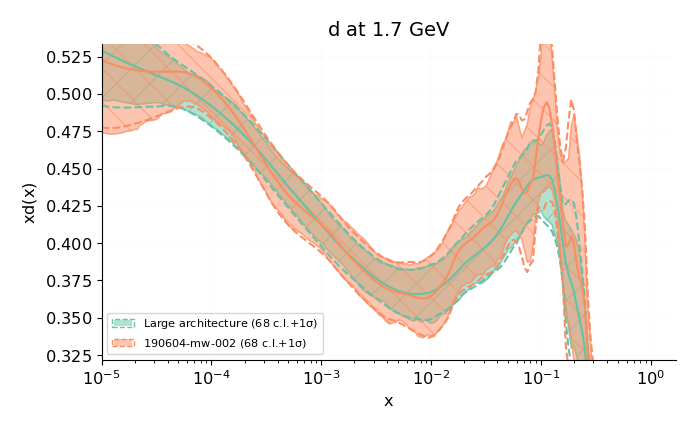
\includegraphics[width=0.8\textwidth]{level0onlargearch.png}
    \caption{
        Figure showing an example of the level 0 PDF being smoother than input,
        suggesting that the wiggly behaviour may not be translated to the observables.
        Large architecture is the level 0 closure, 190604-mw-002 is the large arch.
        fit to data.
        }
    \label{fig:dsmoothpdf}
\end{figure}

From this test we are would be persuaded that the underlying PDF was just fitting
flat directions in the loss and that the fluctuations in the PDF shouldn't be
taken too seriously.

One other notable thing is that the spread on replicas, despite being a level 0
PDF, seems quite high. This also is indicating a rather substantial methodological
error.

\begin{figure}[!h]
    \centering
    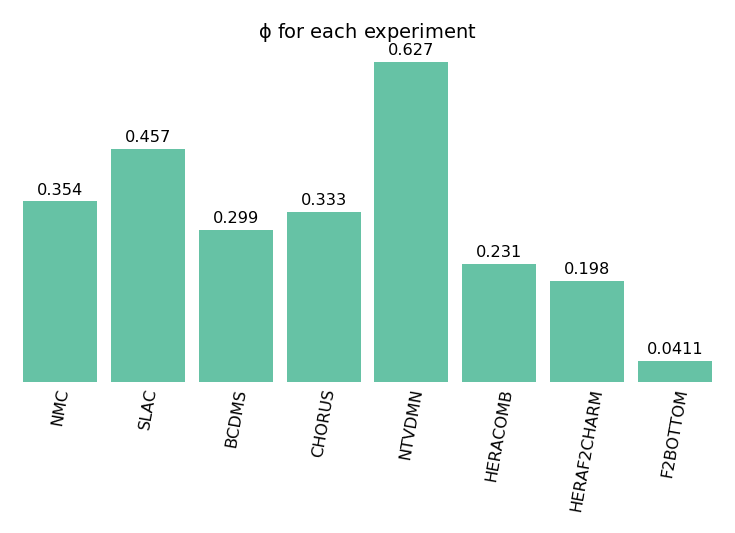
\includegraphics[width=0.8\textwidth]{closure_fitunderlyinglaw_closure_plot_phi.png}
    \caption{
        Figure showing the high values of phi (sqrt(Variance)) per data point
        suggesting high methodological error.
        }
    \label{fig:lev0methoderr}
\end{figure}

\subsubsection*{Closures with different level 1 shift}

A second sanity check was to run two different closures changing nothing but the
seed used to generate the level 1 shifts on the pseudodata. This was a test I
wanted to run to check how important it was that we considered two closures ran
not only on the same datasets but also with the same level 1 noise. In other
words, how robust are the statistical estimators on the level 1 noise? In particular
we added bootstrap sampling to some of the statistical estimators and it would
be good to know if the errorbar given by a bootstrap represents the distribution
under different level 1 shifts.

The full report can be found here:
\href{https://vp.nnpdf.science/mbcTUd6-TQmQFvaGd37bkg==}{\bf{report}}. In particular
one will note that the variance is unchanged within statistics as you would expect
but the bias and the $\dcs$ both appear to depend heavily on the level 1 noise.

This serves as a warning that the closure tests should be ran with the same level
1 data if they are to be compared.


\subsubsection*{Closures on \texttt{MSTW2008nlo68cl}}

Now we take the smooth \texttt{MSTW2008nlo68cl} as input. We fit this
with both the conservative architecture, roughly corresponding to the number of
parameters used in NNPDF3.1, and the larger architecture found by the hyperopt
routine. The objective here is to see if we can use the closure test estimators
to distinguish and discriminate between the two fits.

All, full reports can be found on the
\href{https://www.wiki.ed.ac.uk/display/nnpdfwiki/n3fit+closure+results}{\bf{Wiki}}.

One notable thing which we noticed here, which motivated the further investigation
in section \ref{sec:estimators}, was that the total $\dcs$ for the larger architecture
actually looks a bit better than for the baseline. With the old understand
the naive conclusion here would be that across the whole fit the larger architecture
is closer to the perfect fit since $\dcs$ is closer to 0, see figure \ref{fig:no_test_dcs}.

\begin{figure}[!h]
    \centering
    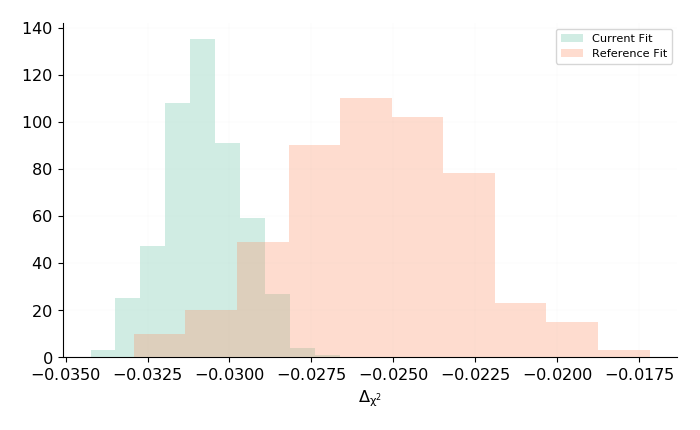
\includegraphics[width=0.8\textwidth]{plot_delta_chi2_notest.png}
    \caption{
        Figure showing that the global $\dcs$ looks better for the reference
        fit, which in this case refers to the larger architecture.
        }
    \label{fig:no_test_dcs}
\end{figure}

We now understand that $\dcs$ on it's own doesn't actually tell us how well
the fit is reproducing the underlying law, and instead when combined with bias
can tell us something about where the fit sits in relation to the shift and the
underlying law.

Comparing the total bias of the two fits in table \ref{tab:totbiasnotest} we
see that the large architecture has a bias over twice that of the baseline architecture.

\begin{center}
    \begin{tabular}{ |c|c| }
     \hline
     baseline arch. & large arch.  \\
     \hline\hline
     0.018 & 0.045 \\
     \hline
    \end{tabular}\label{tab:totbiasnotest}
\end{center}

We can also break this down by experiment, with bootstrapping to see how
stable the values with the ensemble of replicas, and see a real noticable difference
in figure \ref{fig:no_test_bias_exp}. The $\dcs$ is the real smoking gun that
the larger architecture is unable to reproduce the underlying law, both
globally and consistently across datasets.

\begin{figure}[!h]
    \centering
    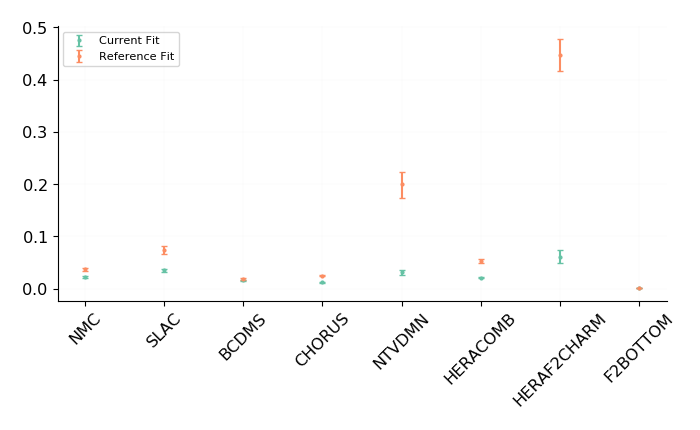
\includegraphics[width=0.8\textwidth]{plot_fits_bootstrap_bias_notest.png}
    \caption{Figure showing the breakdown of bias by experiment}
    \label{fig:no_test_bias_exp}
\end{figure}

\subsubsection*{Closures with a TEST set}

At this point the larger architecture has already shown to have an increase
of bias and variance both globally and consistently across datasets, and so
we already would have concluded that the baseline architecture is preferable.

The final thing which would be interesting to see is the same comparison but
this time including a new experiment called TEST which doesn't get included
in either the training or validation sets. This of course is leading up to
being able to calculate the generalisation error which was proposed in section
\ref{sec:estimators}.

The TEST set is constructed by choosing datasets which cover the same kinematics
as at least one other dataset. The datasets which were chosen for the TEST set
in the DIS only fit here are listed in \ref{tab:deftestset}.

\begin{center}
    \begin{tabular}{ |c| }
        \hline
        Dataset name \\
        \hline\hline
        NMC \\
        BCDMSP \\
        BCDMSD \\
        HERACOMBNCEP460 \\
        H1HERAF2B \\
        \hline
   \end{tabular}\label{tab:deftestset}
\end{center}

The large architecture looks worse by pretty much all accounts
with this new fit, but of particular interest are the various TEST set numbers
which are tabulated in table \ref{tab:testsetnumbers}.

\begin{center}
    \begin{tabular}{ |c|c|c| }
        \hline
        Estimator Name & baseline value & large arch. value \\
        \hline\hline
        Bias & 0.074& 0.198\\
        sqrt(Variance) & 0.4088 & 0.9628\\
        $\dcs$ & 0.071& 0.21\\
        \hline
   \end{tabular}\label{tab:testsetnumbers}
\end{center}

The spread of replicas in the test set for the large architecture is almost
as large as the spread of pseudodata. We then see that both $\dcs$ and Bias are
more than twice the values for the baseline architecture.

\subsection{Summary}

\begin{itemize}
    \item The closure test estimators can discriminate successfully between architectures
    \item If we define a test set, we can get the generalization error and in
        turn decompose this into the estimators, to understand how the fit
        performs data not seen.
    \item Potentially the \hyperopt\ routine could be performed to minimise the
        test set Bias. This would open some questions, such as how does this
        affect the other estimators and would this depend too heavily on the input
        PDF and chosen test set. Of course those questions can be answered with
        further closure tests and hyper parameter scans with different settings.
\end{itemize}
